\documentclass[11pt]{report}
\usepackage[pdftex]{graphicx}
\usepackage{henrian-more}
\usepackage{subfig}
\usepackage{booktabs}
\usepackage{rotating}
\usepackage{float}

\makeHeaders{Machine Learning: Homework 2}


\begin{document}

\begin{itemize}
  \item \textbf{Email}: chrisbrown@utexas.edu
  \item \textbf{EID}: chb595
\end{itemize}

\section{Algorithm}

The PCA (Principal Component Analysis) algorithm is pretty straightforward, and the MATLAB implementation closely follows the general instructions. My \texttt{hw2FindEigendigits} function is a short 12 lines of code, and could be much shorter by embedding many of the functions. One complication (due to the original version of the assignment) was that sometimes the width of the matrix did not exceed the number of original dimensions of the data (784 in our case), and since the function was required to return a matrix the same size as the input image data, I found that padding it out with zeros was a suitable solution. In those cases where the number of training images was less than 748, truncating the eigenvector matrix to match that number was easy enough. Also, the assignment noted that the eigenvector matrix would need to be sorted by eigenvalues, but MATLAB's \texttt{eig} does that automatically, and only a reverse is needed. However, in line with the assignment, I still sort the eigenvalues and return the corresponding eigenvectors. I have produced a sampling of eigenvectors in Figure \ref{fig:100eigenvectors} for different amounts of training data. The first few eigenvectors of each group seem intuitively reasonable, vaguely resembling the `0' shape that covers much of the space used by a digit. However, after the first ten or so, they seem to become random and hardly distinguishable.

\begin{figure}[H]
  \centering
  \subfloat[Using 25 training images]{
    \makebox[0.3\textwidth]{
      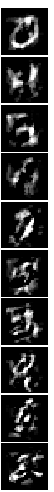
\includegraphics[height=0.3\textwidth]{../plots/eigenvectors-25.pdf}
    }
  }
  \subfloat[Using 100 training images]{
    \makebox[0.3\textwidth]{
      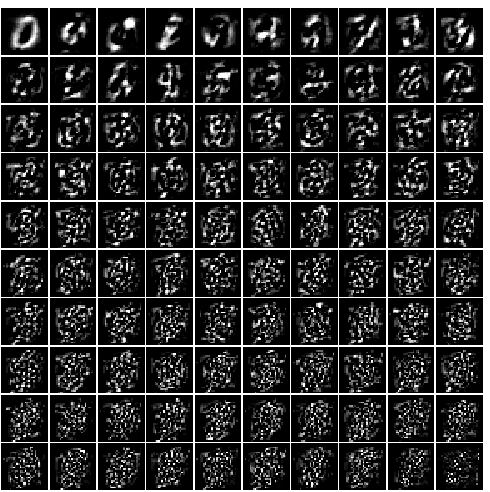
\includegraphics[height=0.3\textwidth]{../plots/eigenvectors-100.pdf}
    }
  }
  \subfloat[Using all training data (60,000 images)]{
    \makebox[0.3\textwidth]{
      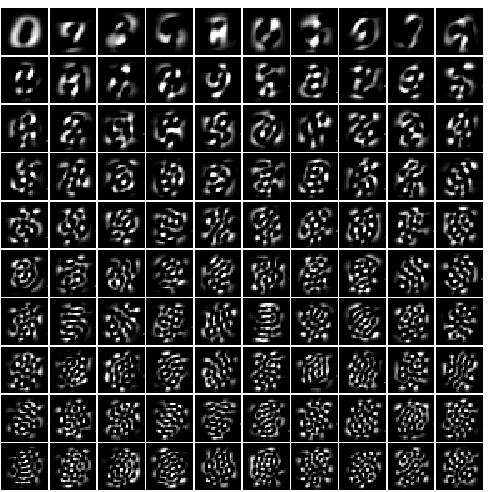
\includegraphics[height=0.3\textwidth]{../plots/eigenvectors-60000.pdf}
    }
  }
  \caption{The first 10 or 100 eigenvectors (ordered by rows, not columns)}
  \label{fig:100eigenvectors}
\end{figure}

\section{Evaluation}

I tried out four basic evaluation metrics:

\begin{itemize}
  \item kNN (k = 1) \hfill (kNN: k-Nearest Neighbors)
  \item kNN (k = 10) -- majority vote
  \item kNN (k = 10) -- weighted vote
  \item Cosine similarity
\end{itemize}

Most of the computation time is spent evaluating each point relative to the training data. It's easy to project all the training/labeled data and the test data into the space of reduced dimensionality quickly, so I only had to do that once per choice of evaluation metric, number of training images, and number of top eigenvectors. But to evaluate a large group of test data, the algorithm would evaluate each one in term, analyzing the entirety of the training data to find the closest points.
If speed was an issue, we could probably do some preprocessing on the training data to assign different regions of the PCA space certain labels, and then the test points could be queried against these regions, instead of all 60,000 training points.

At first, I used kNN with k = 10 and took the most popular label from the resulting list. This ended up being slightly better than kNN with k = 1, since in some cases you can have a particularly sloppy `4' that looks a \emph{lot} like some other specific and also very sloppy `9,' but in general looks more like a `4' than a `9,' based on several other digits. That is, it takes out some of the anomalies. The advantages of this diminishes as we gain more training images, as the PCA space becomes more saturated with examples. But then I realized that this was naive, and that since the \texttt{knnsearch} function returns distances as well as a simple indexation, I could average the distance to all the `4' matches in the top 10, and all the `9' matches, for example, and take the shortest of those. This turned out not to really make a difference, but since it seemed to make more sense, I proceeded to use this metric (weighted kNN, k = 10) for the final analysis.

Cosine similarity (using \texttt{pdist2}, not the cosine option of \texttt{knnsearch}), gave me decent results, but it wasn't nearly as fast or successful as \texttt{knnsearch} using euclidean distances. Also, MATLAB warned me that my data did not seem entirely suitable for the cosine similarity metric, which is probably true.

See Figure \ref{fig:metrics} for a comparison of these different metrics over a limited number of test images. (I only used 200 images in these plots, since evaluating 10,000 takes quite a bit of time.)

\begin{figure}[H]
  \centering
  \subfloat[1-NN]{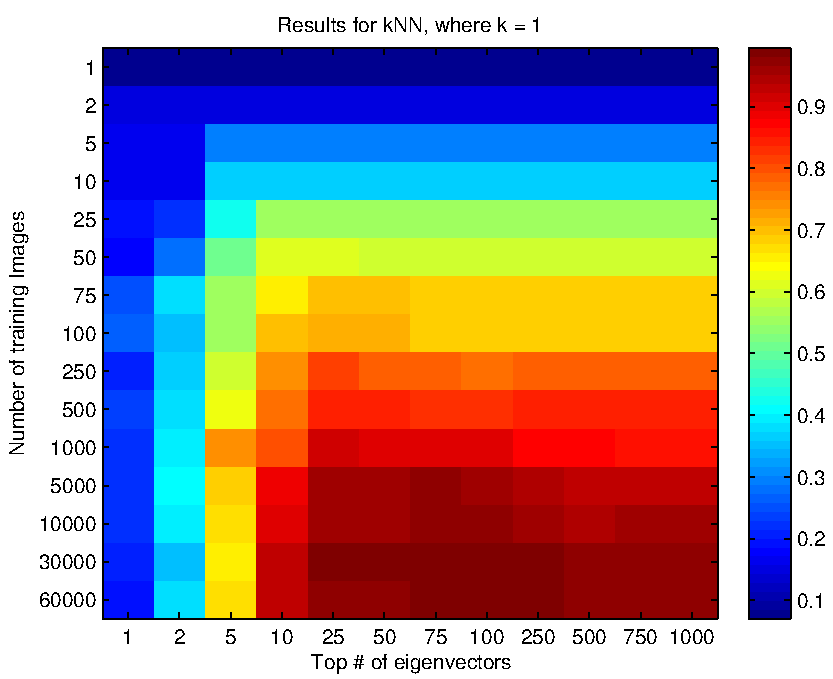
\includegraphics[width=0.5\textwidth]{../plots/metrics-1nn.pdf}}\hfil
  \subfloat[10-NN majority vote]{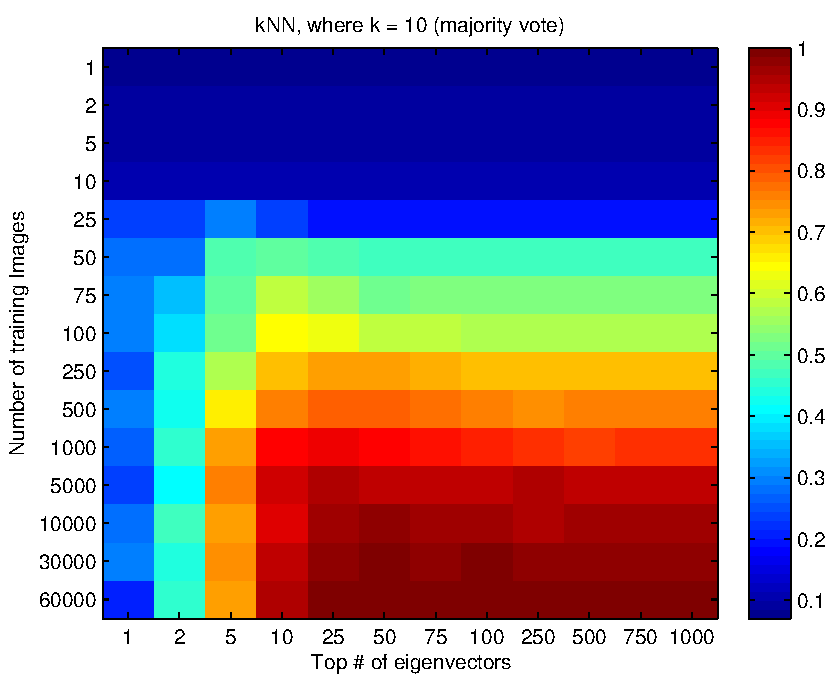
\includegraphics[width=0.5\textwidth]{../plots/metrics-10nn-vote.pdf}}

  \subfloat[10-NN weighted]{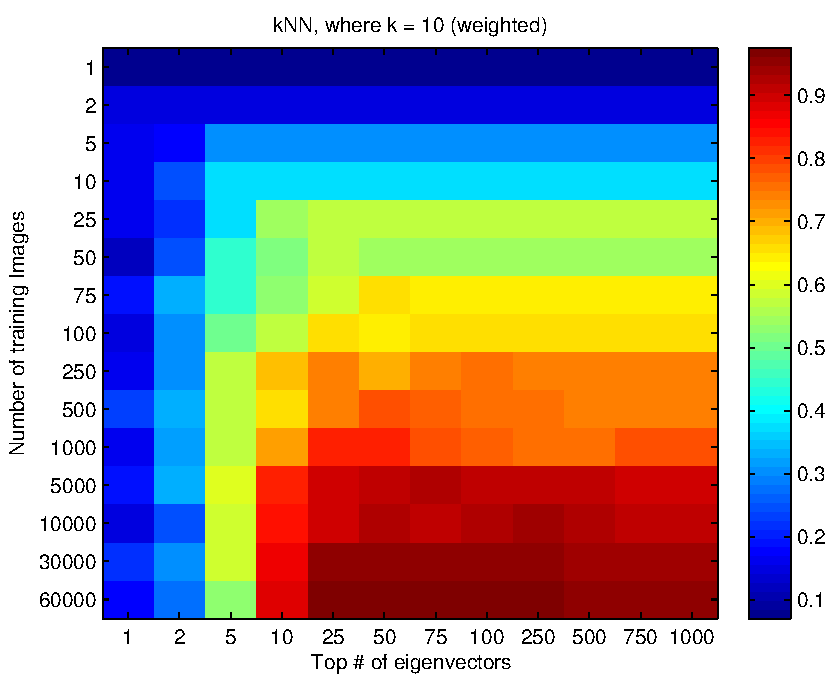
\includegraphics[width=0.5\textwidth]{../plots/metrics-10nn-weighted.pdf}}\hfil
  \subfloat[Cosine similarity]{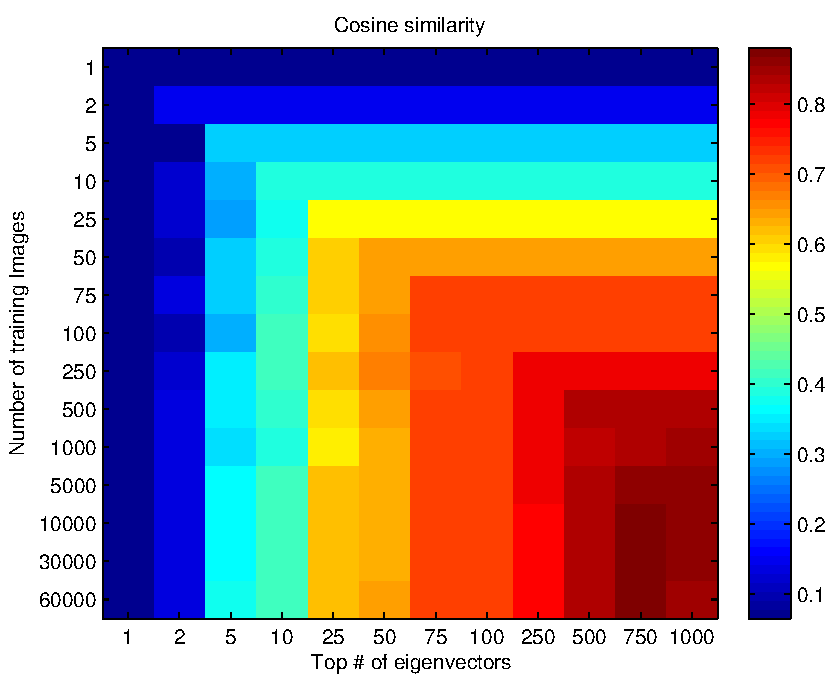
\includegraphics[width=0.5\textwidth]{../plots/metrics-cosine.pdf}}

  \caption{Evaluation metrics. The hotter the color, the more accurate the combination of top eigenvectors and number of test images. Please note that these may look blurry due to the non-standard way Mac OS X Preview renders small images. Use Adobe Acrobat to see a correct rendering.}
  \label{fig:metrics}
\end{figure}

\section{Results}


There are two variables we can plot accuracy on: the number of top eigenvectors (the dimensionality of the eigenspace), and the number of training images. I do this for different portions of the test data:

\begin{figure}[H]
  \centering
  \subfloat[Easy 5,000]{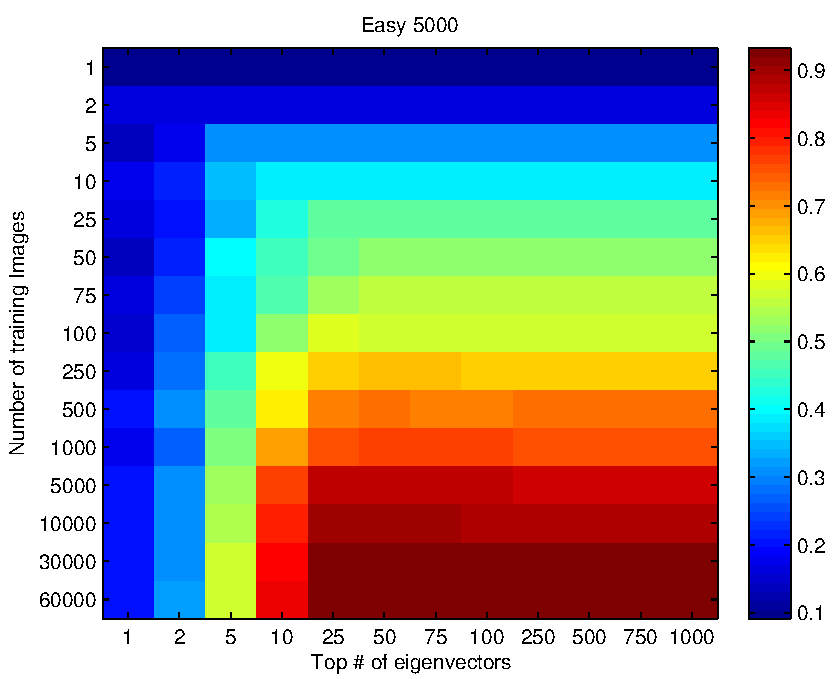
\includegraphics[width=0.5\textwidth]{../plots/results-easy-5000.pdf}}\hfil
  \subfloat[Hard 5,000]{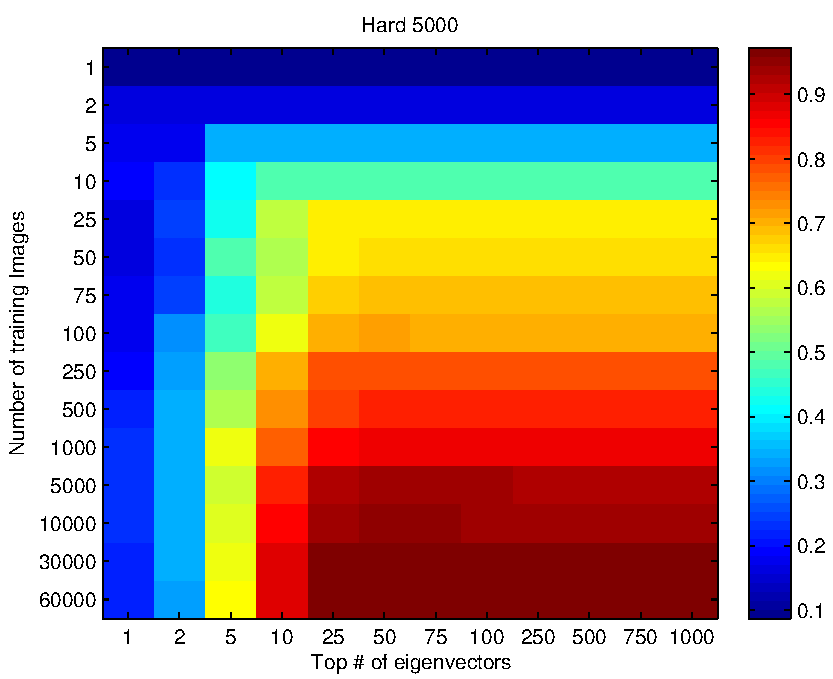
\includegraphics[width=0.5\textwidth]{../plots/results-hard-5000.pdf}}

  \subfloat[All 10,000]{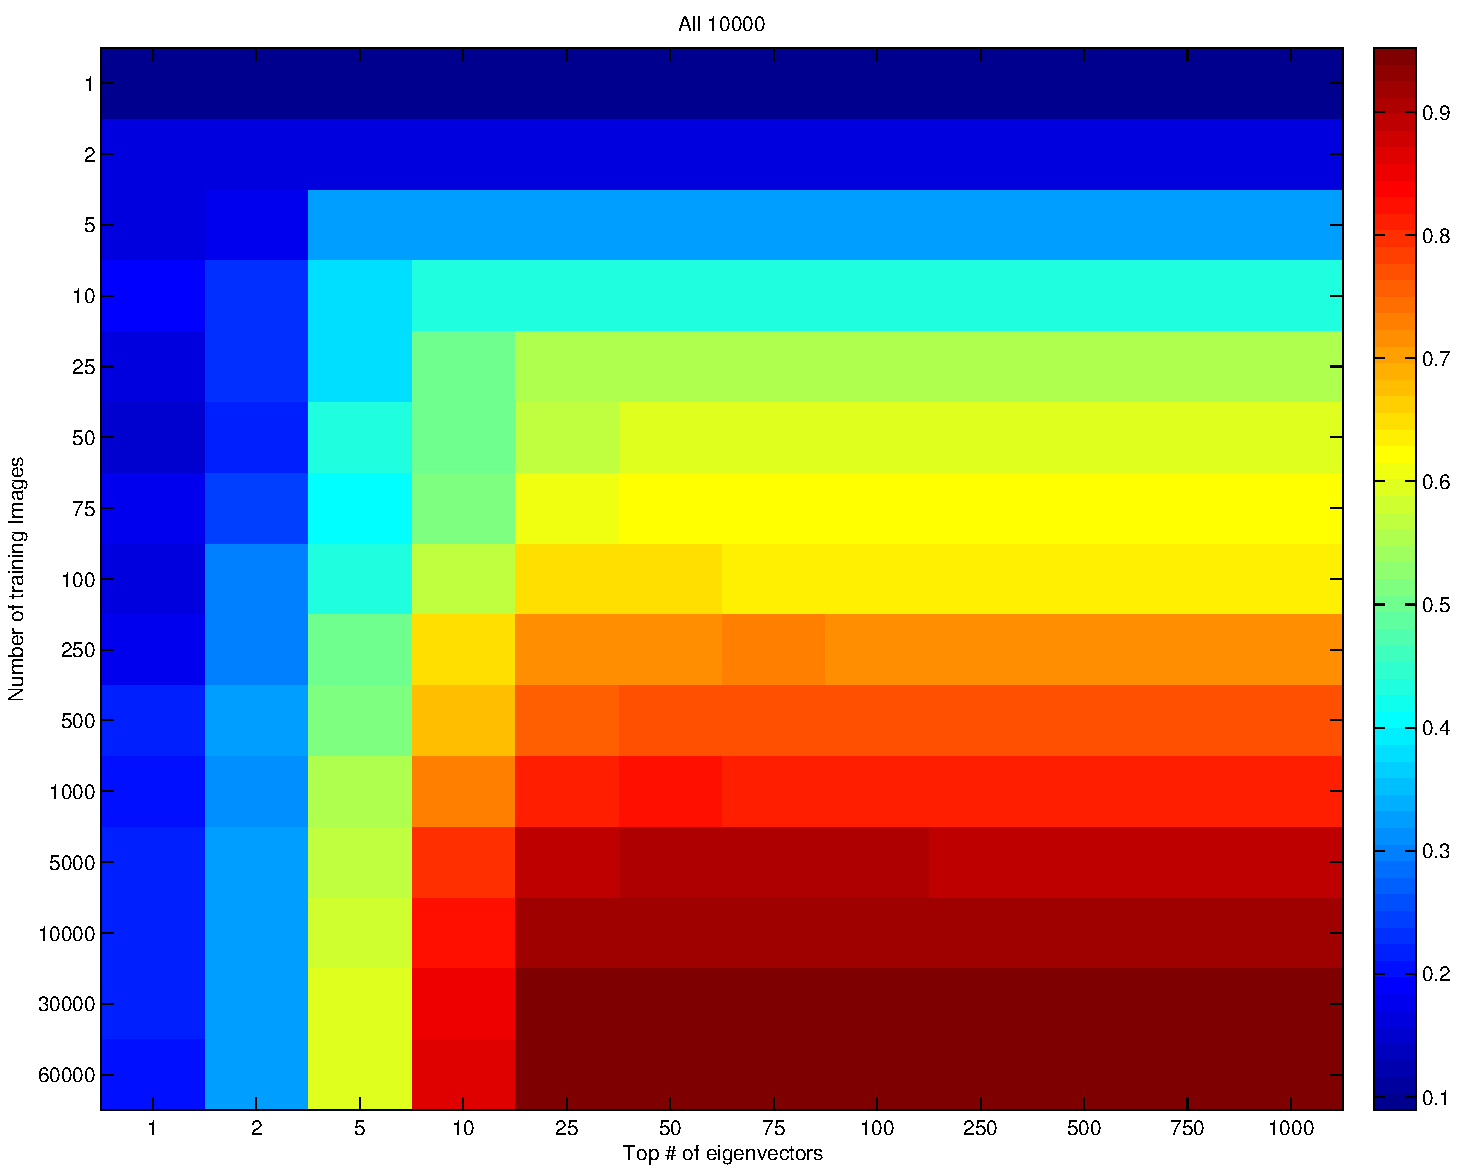
\includegraphics[width=\textwidth]{../plots/results-all-10000.pdf}}
  \caption{Results}
  \label{fig:results}
\end{figure}

We see that we can get pretty good results for as few as 500 training images while using just the top 50 eigenvectors. Perhaps the most interesting thing about these graphs is that for fewer training images, in the 100-10,000 range, it helps to truncate the eigenvectors, `de-noising' the data when transforming it into the PCA space, in a way. However, this advantage falls off as we simply use more and more training images (which is just another way of reducing noise in the training dataset).


Overall, we achieved up to 93.28\% accuracy on the ``easy'' images (using the full test set, and the top 50 eigenvectors), and 97.18\% on the ``hard'' images. I didn't visually compare the different sets of the last 5,000 and first 5,000 of the 10,000 training images, so I must have accidentally put the last 5,000 results into the `easy' results. That or the assignment got the ordering backwards, because one would expect lower accuracy for the ``harder'' images. The top accuracy for the full 10,000, measured in a separate run, is predictably the mean of the other top accuracies: 95.23\%. The full table for all 10,000 is in Figure \ref{fig:tabled}.

\begin{figure}[H]
  \begin{sideways}\ \ \ \ \ Number of Training Images\end{sideways}
  \begin{small}
    \begin{tabular}[b]{@{}r c c c c c c c c c c c c@{}}
      \toprule
      \multicolumn{13}{c}{Top \# of Eigenvectors} \\
      ~ & 1 & 2 & 5 & 10 & 25 & 50 & 75 & 100 & 250 & 500 & 750 & 1000 \\
      \midrule
            1 & 0.089 & 0.089 & 0.089 & 0.089 & 0.089 & 0.089 & 0.089 & 0.089 & 0.089 & 0.089 & 0.089 & 0.089 \\
            2 & 0.161 & 0.161 & 0.161 & 0.161 & 0.161 & 0.161 & 0.161 & 0.161 & 0.161 & 0.161 & 0.161 & 0.161 \\
            5 & 0.158 & 0.175 & 0.324 & 0.324 & 0.324 & 0.324 & 0.324 & 0.324 & 0.324 & 0.324 & 0.324 & 0.324 \\
           10 & 0.187 & 0.225 & 0.379 & 0.433 & 0.433 & 0.433 & 0.433 & 0.433 & 0.433 & 0.433 & 0.433 & 0.433 \\
           25 & 0.162 & 0.229 & 0.381 & 0.502 & 0.561 & 0.561 & 0.561 & 0.561 & 0.561 & 0.561 & 0.561 & 0.561 \\
           50 & 0.146 & 0.219 & 0.439 & 0.505 & 0.567 & 0.590 & 0.590 & 0.590 & 0.590 & 0.590 & 0.590 & 0.590 \\
           75 & 0.172 & 0.244 & 0.409 & 0.517 & 0.606 & 0.623 & 0.621 & 0.621 & 0.621 & 0.621 & 0.621 & 0.621 \\
          100 & 0.166 & 0.296 & 0.428 & 0.566 & 0.642 & 0.643 & 0.638 & 0.639 & 0.639 & 0.639 & 0.639 & 0.639 \\
          250 & 0.178 & 0.304 & 0.499 & 0.645 & 0.717 & 0.723 & 0.724 & 0.720 & 0.720 & 0.720 & 0.720 & 0.720 \\
          500 & 0.212 & 0.327 & 0.520 & 0.674 & 0.756 & 0.773 & 0.773 & 0.771 & 0.773 & 0.772 & 0.772 & 0.772 \\
         1000 & 0.200 & 0.306 & 0.561 & 0.728 & 0.805 & 0.823 & 0.817 & 0.816 & 0.812 & 0.810 & 0.810 & 0.810 \\
         5000 & 0.214 & 0.329 & 0.567 & 0.802 & 0.897 & 0.904 & 0.903 & 0.900 & 0.898 & 0.896 & 0.896 & 0.896 \\
        10000 & 0.214 & 0.323 & 0.575 & 0.823 & 0.921 & 0.922 & 0.922 & 0.917 & 0.916 & 0.915 & 0.915 & 0.915 \\
        30000 & 0.212 & 0.324 & 0.593 & 0.850 & 0.941 & 0.946 & 0.947 & 0.946 & 0.943 & 0.942 & 0.943 & 0.943 \\
        60000 & 0.210 & 0.325 & 0.601 & 0.859 & 0.948 & \textbf{0.952} & 0.951 & 0.951 & 0.950 & 0.949 & 0.949 & 0.000 \\
      \bottomrule
    \end{tabular}
  \end{small}
  \caption{Results Table}
  \label{fig:tabled}
\end{figure}

The most interesting observation was that less eigenvectors give better results, but less notably so with more training images. But another interesting problem was the matrix manipulation to average the distances from \texttt{knnsearch} while grouping by label. This would be called 1,800,000 times for the full evaluation of the 10,000 test images alone, so I wanted to avoid a for-loop if possible. So I created a matrix of mostly zeros from the list of labels returned by \texttt{knnsearch}, which, when multiplied by the distances, would sum the distances for each label, returning a vector as long as the number of labels. Then I just divided by the vector-sum of that multipler matrix, and had my averages.

\end{document}


What happens if you trim the vector down and only use the top n eigenvectors? How accurately can you classify using nearest neighbor using cosine similarity? Plot figures showing the accuracy as the number of training points increases, and as the number of eigenvectors increases.

Must the images be centered exactly? what if they aren't?

What happens if you trim the vector down and only use the top n eigenvectors? How accurately can you classify using the method on page 21 of the lecture notes using the Euclidean distance metric? Plot figures showing the accuracy as the number of training points increases, and as the number of eigenvectors increases.

Write, review, and submit a brief report detailing what you did, how well it worked, and something interesting that you learned. At the beginning of your report include your email address and EID in addition to your name. Also submit your code. Submit using turnin to hychyc07. This is hw2.

